
%\pagestyle{myheadings}
%\markright{{\large ME 4140 Fall 2019---The Robotic Operating System}}


% Tennessee Technological University
% ME4140 - Fall 2016 - Fall2017 - Fall 2020 
% Tristan Hill - September 11, 2020
% Module 2 - Linux Basics

%\textwidth=6.5in
%\topmargin=-0.5in
%\textheight=9.25in
%\hoffset=-0.5in
%\footskip=0.2in


\documentclass[fleqn]{beamer}                         % for presentation (has nav buttons at bottom)
%\documentclass[handout]{beamer}  % for handout 
\usepackage{beamerthemesplit}
\usepackage{amsmath}
\usepackage{listings}
\usepackage{multicol}
\usepackage{framed}

\usepackage{graphicx}
\usepackage{keystroke}



\beamertemplateballitem

% custom colors
\definecolor{TTUpurple}{rgb}{0.3098, 0.1607, 0.5176} % TTU Purple (primary)
\definecolor{TTUgold}{rgb}{1.0000, 0.8666, 0.0000} % TTU Gold (primary) 
\definecolor{mygray}{rgb}{.6, .6, .6}
\definecolor{mypurple}{rgb}{0.6,0.1961,0.8}
\definecolor{mybrown}{rgb}{0.5451,0.2706,0.0745}
\definecolor{mygreen}{rgb}{0, .39, 0}
\definecolor{mypink}{rgb}{0.9960, 0, 0.9960}

% color commands
\newcommand{\R}{\color{red}}
\newcommand{\B}{\color{blue}}
\newcommand{\BR}{\color{mybrown}}
\newcommand{\K}{\color{black}}
\newcommand{\G}{\color{mygreen}}
\newcommand{\PR}{\color{mypurple}}
\newcommand{\PN}{\color{mypink}}
\newcommand{\OR}{\color{TTU}}
\newcommand{\GD}{\color{TTUgold}}

% beamer colors
\setbeamercolor{palette primary}{bg=TTUpurple,fg=TTUgold}
\setbeamercolor{palette secondary}{bg=black,fg=TTUgold}
\setbeamercolor{palette tertiary}{bg=black,fg=TTUpurple}
\setbeamercolor{palette quaternary}{bg=TTUgold,fg=black}
\setbeamercolor{structure}{fg=TTUpurple} % itemize, enumerate, etc
\setbeamercolor{section in toc}{fg=TTUpurple} % TOC sections

\newcommand{\Lagr}{\mathcal{L}} % lagrangian

\newcommand{\hspcu}{\underline{\hspace{20mm}}} % large horizontal space w underline
\newcommand{\vspccc}{\vspace{6mm}\\} % large vertical space
\newcommand{\vspcc}{\vspace{4mm}\\}   % medium vertical space
\newcommand{\vspc}{\vspace{2mm}\\}     % small vertical space

\newcommand{\hspcccc}{\hspace{10mm}} % large horizontal space
\newcommand{\hspccc}{\hspace{6mm}} % large horizontal space
\newcommand{\hspcc}{\hspace{4mm}}   % medium horizontal space
\newcommand{\hspc}{\hspace{2mm}}     % small horizontal space

% windows logo
% Lower the picture a little to match the text baseline
\newcommand{\WindowsLogo}{\raisebox{-0.1em}{%
  
\includegraphics[height=0.8em]{win_logo}}}
\newcommand{\WinKey}{\keystroke{\WindowsLogo}}

\newcommand{\CTRL}{\raisebox{-0.1em}{Ctrl}}
\newcommand{\CTRLKey}{\keystroke{\CTRL}}

\newcommand{\ALT}{\raisebox{-0.1em}{Alt}}
\newcommand{\ALTKey}{\keystroke{\ALT}}

\newsavebox{\mybox} % custom box

\newcommand{\MNUM}{2\hspace{2mm}} % Module number
\newcommand{\TNUM}{---\hspace{2mm}} % Topic number - single topic for now
\newcommand{\moduletitle}{Linux Basics} % Titles and Stuff
%\newcommand{\topictitle}{---} 

\newcommand{\sectiontitleI}{What is Linux?} % More Titles and Stuff
\newcommand{\sectiontitleII}{A Brief History}
\newcommand{\sectiontitleIII}{Keyboard Shortcuts}
\newcommand{\sectiontitleIV}{The Terminal}
\newcommand{\sectiontitleV}{Tutorial 2 - Install ROS Melodic}

\title{ME4140 - ROS Workshop}

\author{Mechanical Engineering\vspc Tennessee Technological University}

\date{Tristan Hill, Lecturer}

\begin{document}

\lstset{language=MATLAB,basicstyle=\ttfamily\small,showstringspaces=false}

\frame{\titlepage \center\begin{framed}\Large \textbf{Module \MNUM - \moduletitle}\end{framed} \vspace{5mm}}

% Section 0 - Outline
\frame{
	
	\large \textbf{Module \MNUM - \moduletitle} \vspace{3mm}\\
	
	\begin{itemize}
	
		\item \sectiontitleI    \vspc % Section I
		\item \sectiontitleII 	\vspc % Section II
		\item \sectiontitleIII 	\vspc %Section III
		\item \sectiontitleIV 	\vspc %Section IV
		\item \hyperlink{sectionV}{\sectiontitleV} \vspc %Section IV	
	
	\end{itemize}

}

\section{\sectiontitleI}

	% Section I - Frame I
	\frame{ \small
		\frametitle{\sectiontitleI}
		
\begin{itemize}
		\item {\it Just like Windows, iOS, and Mac OS, Linux is an operating system. In fact, one of the most popular platforms on the planet, Android, is powered by the Linux operating system. An operating system is software that manages all of the hardware resources associated with your desktop or laptop. To put it simply, the operating system manages the communication between your software and your hardware. Without the operating system (OS), the software wouldn?t function.} - \href{https://www.linux.com/what-is-linux/}{LINUX.COM}  \vspc
        
            \end{itemize}
	}

	% Section I - Frame II
	\frame{ \small
		\frametitle{\sectiontitleI}
			Ubuntu is a {\B distribution} of Linux. But there are many others. 
            \begin{itemize}
                \item 
                \item 
                \item 
            \end{itemize} 

	}
		
\section{\sectiontitleII}	

	\frame{ \small
		\frametitle{\sectiontitleII}
			Once upon a time in California ...
            \begin{itemize}
                \item Unix was developed at Bell Labs (AT\&T) 
                \item Linus Torvalds   
                \item read the whole story \href{https://en.wikipedia.org/wiki/History_of_Linux}{here} or \href{https://www.bell-labs.com/var/articles/invention-unix/}{here}
            \end{itemize} 

	}
		


\section{\sectiontitleIII}	
	% Section III - Frame I
	\frame{ \small
		\frametitle{\sectiontitleIII}
		Press \WinKey and type {\it Keyboard Shortcuts} to list shortcuts in Ubuntu.
		
		\begin{multicols}{2}
		
		\renewcommand{\arraystretch}{1.4}
		\begin{tabular}{|c|c|}\hline
			Function & Shortcut \\ \hline
			Launcher &\WinKey  \\
			New Terminal &\CTRLKey+\ALTKey+T \\
			Abort Process &\\
		    Switch Windows &\\
			Close Window & \\
			Rename &\\
			New Folder & \\ \hline						
		\end{tabular}
			
		\hspace{10mm}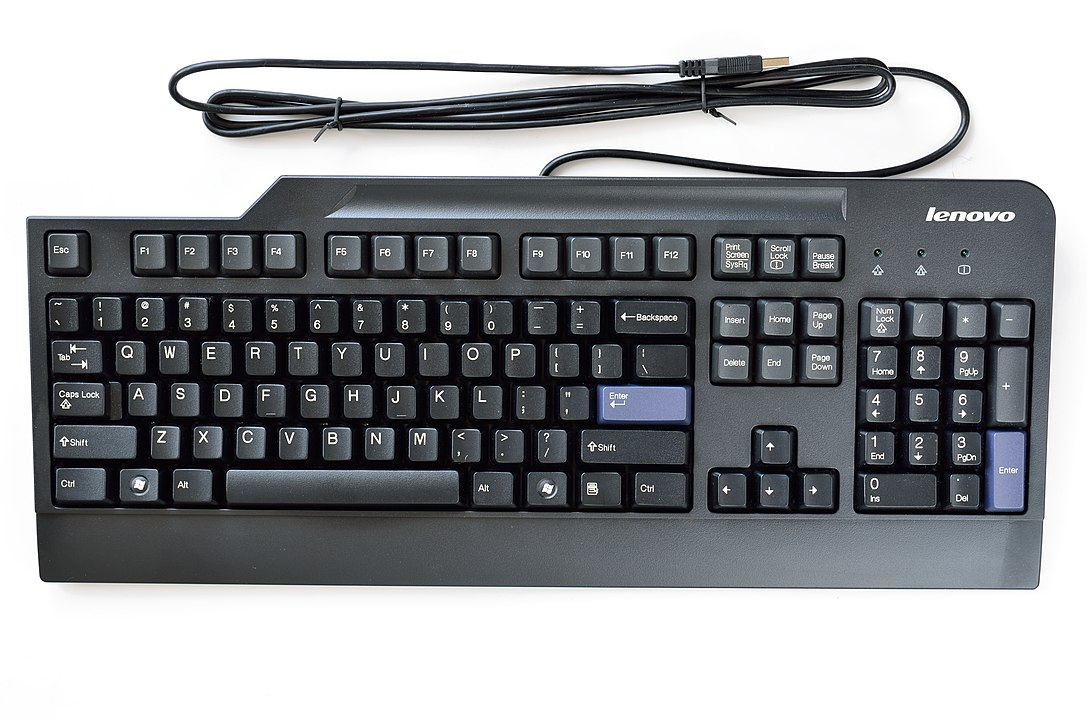
\includegraphics[scale=.10]{lenovo_keyboard.jpg} 
       	       
        \end{multicols}

	}      
	
\section{\sectiontitleIV}	
	% Section IV - Frame I
	            \frame{ \small
		\frametitle{\sectiontitleIV}    
          The {\it Terminal} is a text based interface to the computer.\vspace{2mm}\\ Press CTRLKey+\ALTKey+T to open a new terminal. \vspace{3mm}\\      
                \begin{multicols}{2}
		



		\renewcommand{\arraystretch}{1.4}
		\begin{tabular}{|c|c|}\hline
				Function & Command \\ \hline
			 Change Directory & cd  \\ 
			List Directory & ls \\  
			Copy File& cp \\ 
			Remove File& rm  \\ 
			Abort Process& \CTRLKey + C  \\ 
			Clear Terminal& \CTRLKey + L  \\ \hline
				
		\end{tabular}
			
		\hspace{10mm}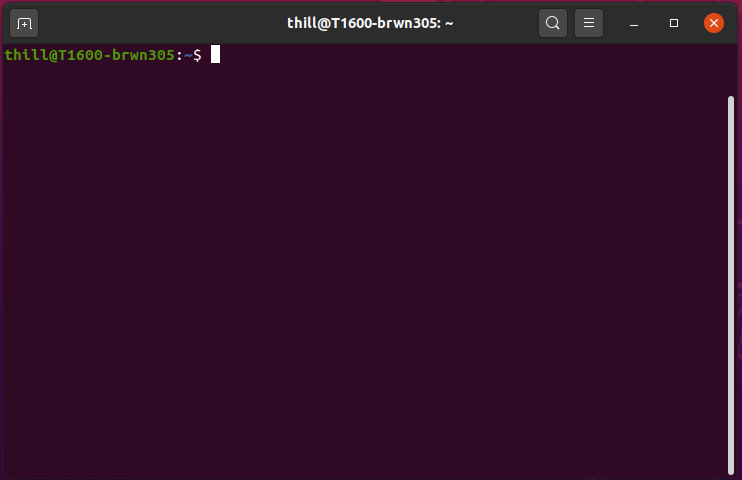
\includegraphics[scale=.20]{ubuntu_terminal.png}  
       	       
        \end{multicols}

       	                       
                
		}
		


\section{\sectiontitleV}	
	% Section V - Frame I
	            \begin{frame}[label=sectionV] \small
		\frametitle{\sectiontitleV}    
	
 \setbeamertemplate{itemize items}[triangle]
                \begin{itemize}

					\item {\bf Overview:} ROS runs on Linux! Your first exercise is to setup your computer so that you can begin learning ROS. 		

					\item {\bf Assignment:} Complete the tutorial in the document {\it tutorial2\_install\_ROS.pdf} on ilearn. Your new system must have ROS Melodic installed.
                    
                    \item {\bf Deliverable:} Write a one to two paragraph summary of what you accomplished and what you struggled with the most. Include an image of a terminal after the {\it roscore} command. 
    
                    \item {\bf Next Week:} After completion of Module 2, you will be ready to start using ROS. You will begin with a Turtlebot3 robot platform in a Gazebo simulator. \vspc
                    
                    
    
                    
                \end{itemize}
		\end{frame}

\end{document}


